\section{Derivation of equations in the main text} \label{app:eq}


\subsection{Different growth rate}

I write below the equations deriving equation \ref{eq:growth}.

For the input cosmology, we define:
\begin{equation}
 P(z,k) = P_\star(k) \left[ \frac{D(z)}{D_\star} \right]^2 ~,
\end{equation}
where $D(z)$ is the growth factor and $_\star$ means that the quantity is 
evaluated at $z_\star=3$. 

The evolution of the growth factor is quite similar to Einstein-de Sitter 
(EdS), i.e., $D(z) \propto a(z)$, and we define the deviation from that growth 
as follows:
\begin{equation}
 \frac{D(z)}{D_\star} = \frac{a(z)}{a_\star} ~ \eta(z) ~,
\end{equation}
with $\eta_\star=1$ by definition and $\eta(z)=1$ in an EdS universe.

We can then do a Taylor expansion of $\eta(z)$ around $z_\star$:
\begin{align}
 \eta(z_\star+\Delta z) 
  & = 1 + \frac{\partial \eta}{\partial z} 
      \Bigr\rvert_{z_\star} \Delta z                    \nonumber \\
  & = 1 - a_\star^2~\frac{\partial \eta}{\partial a} 
      \Bigr\rvert_{z_\star} \Delta z                    \nonumber \\
  & = 1 + \left( 1 - f_\star \right) \frac{\Delta z}{1+z_\star} ~,
\end{align}
where we have used 
\begin{equation}
 \frac{\partial \eta}{\partial a} \Bigr\rvert_{z_\star} 
  = \frac{a_\star}{D_\star} \frac{\partial (D/a)}{\partial a} 
    \Bigr\rvert_{z_\star}
  = \frac{1}{a_\star} \left( f_\star - 1 \right) ~.
\end{equation}

\begin{figure}[ht]
 \begin{center}
  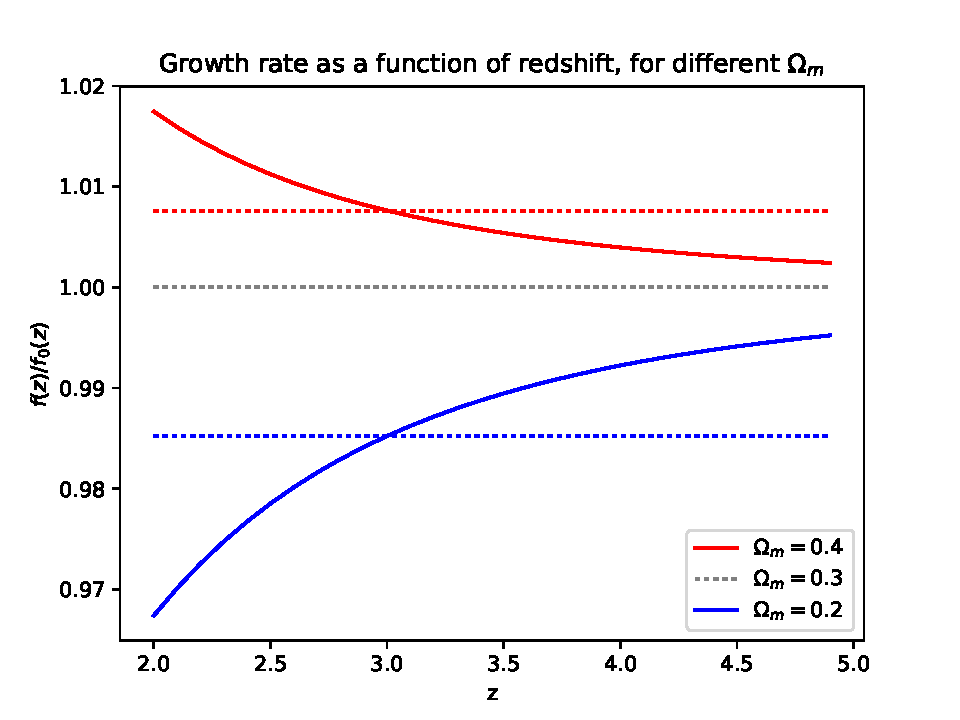
\includegraphics[scale=0.7]{Figures/fz_omega_m}
 \end{center}
 \caption{Logarithmic growth rate, $f(z)$, for different cosmologies.
  Solid lines show the ratio with respect to fiducial ($\Omega_m=0.3$), 
  and dashed lines the value at $z_\star=3$, assumed to be constant in this 
  paper.}
 \label{fig:fz_Om}
\end{figure}

In Figure \ref{fig:fz_Om} we show the difference in growth between different
cosmologies, with the dashed lines showing the residual differences after 
matching at $z_\star=3$.


\subsection{Different expansion rate}

\begin{figure}[ht]
 \begin{center}
  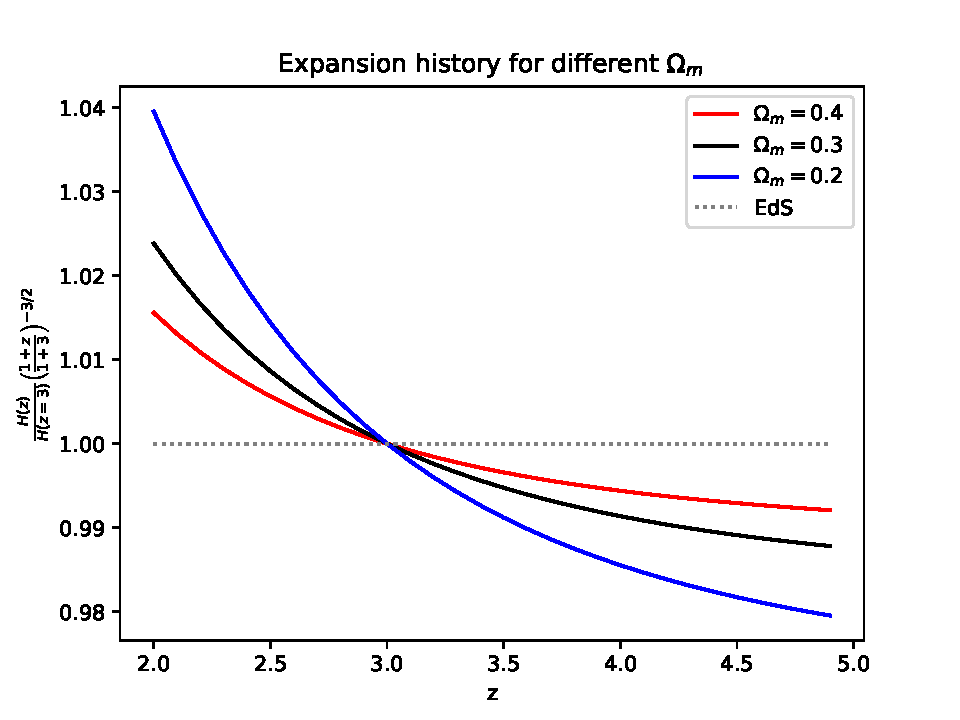
\includegraphics[scale=0.7]{Figures/Hz3_omega_m}
 \end{center}
 \caption{Differences in the expansion rate, $H(z)$, with respect of EdS, 
  for different cosmologies}
 \label{fig:Hz_Om}
\end{figure}

The expansion history at $z>2$ is not quite Einstein-de Sitter (EdS), so 
we might need to worry about the different expansion history of each model
with respect to the fiducial model. 
These differences are shown in Figure \ref{fig:Hz_Om}.

We could do something similar to what we did for the growth factor, and 
define a single parameter (derivative of $H(z)$ at z=3) to parameterize 
that, and add this as an extra likelihood parameter.
